\subsection{Full-Wave Bridge-Network Rectifier With Filter:}

Calculate the Voltage in $R_{L}$ ( $V_{0}$ ), the current in $R_{L}$ ( $I_{0}$ ), the Peak-Voltage ( $V_{p}$ ) at the output of the Transformer $V_{T}$, the Ripple-Voltage ( $\Delta V$ ) and $V_{p}$ - $V_{D}$:

\begin{figure}[H]
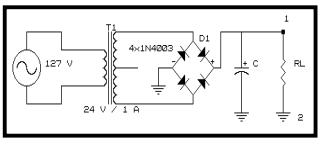
\includegraphics[scale=.9]{fwbnf.png}
\centering \linebreak \linebreak Figure 5.7.0: Full-wave bridge-network rectifier with filter.
\end{figure}

{\bfseries\itshape Where:
\begin{tasks}
\task $R_{L}$ = 100 $\Omega$
\task $V_{D}$ = 0.7 V
\task $V_{T}$ = 12 V
\task f = 120Hz 
\end{tasks}} \hfill

{\bfseries\itshape\color{Maroon}{Solution:}} \hfill \break

\begin{itemize}
\item {\bfseries\itshape\color{Violet}{For peak voltage at the transformer output:}} \hfill \break
{\bfseries\itshape\color{Brown}{
\begin{tasks}
\task Where: $V_{p}$ = $(\ \sqrt{2}\ )(\ V_{rms}\ )$.
\end{tasks}}}
\end{itemize}

\begin{ceqn}
\begin{align}
V_{p} = (\ \sqrt{2}\ )(\ V_{T}\ ) = (\ \sqrt{2}\ )(\ 12 V\ ) = 16.97 V.
\end{align}
\end{ceqn}

\begin{itemize}
\item {\bfseries\itshape\color{Violet}{For $V_{p}$ - ( 2 ) $V_{D}$:}} \hfill \break
\end{itemize}

\begin{ceqn}
\begin{align}
V_{p} - (\ 2\ )(\ V_{D}\ ) = 16.97V - 1.4V = 15.57 V
\end{align}
\end{ceqn}

\begin{itemize}
\item {\bfseries\itshape\color{Violet}{Using 470$\mu F$ capacitor:}} \hfill \break
{\bfseries\itshape\color{Brown}{
\begin{tasks}
\task Where Ripple-Voltage: $\Delta V = (\ \frac{1}{[\ 2\ (\ f\ )(\ R_{L}\ )(\ C\ )\ ]}\ )[\ V_{p} - ( 2 ) V_{D}\ ]:$
\end{tasks}}}
\end{itemize}

\begin{ceqn}
\begin{align}
\Delta V = (\ \frac{1}{[\ 2\ (\ 60Hz\ )(\ 100\Omega\ )(\ 470\mu F\ )\ ]}\ )[\ 15.57 V\ ] = 2.76 V
\end{align}
\end{ceqn}

\begin{itemize}
\item {\bfseries\itshape\color{Violet}{For $V_{0}$:}} \hfill \break
{\bfseries\itshape\color{Brown}{
\begin{tasks}
\task Where $V_{0} = [ 1 - \frac{1}{[\ 2\ (\ f\ )(\ R_{L}\ )(\ C\ )\ ] }][\ V_{p} - ( 2 ) V_{D}\ ]$
\end{tasks}}}
\end{itemize}

\begin{ceqn}
\begin{align}
V_{0} = [ 1 - \frac{1}{[\ 2\ (\ 60Hz\ )(\ 100\Omega\ )(\ 470\mu F\ )\ ] }][\ 15.57 V\ ] = 12.8 V
\end{align}
\end{ceqn}

\begin{itemize}
\item {\bfseries\itshape\color{Violet}{For $I_{0}$:}} \hfill \break
{\bfseries\itshape\color{Brown}{
\begin{tasks}
\task Using Ohm's Law: $I$ = $\frac{V}{R}$.
\end{tasks}}}
\end{itemize}

\begin{ceqn}
\begin{align}
I_{0} = \frac{V_{0}}{R_{L}} = \frac{12.8V}{100\Omega} = 0.128 A.
\end{align}
\end{ceqn}

\pagebreak

\begin{itemize}
\item {\bfseries\itshape\color{Violet}{Using 2200$\mu F$ capacitor:}} \hfill \break
{\bfseries\itshape\color{Brown}{
\begin{tasks}
\task Where Ripple-Voltage: $\Delta V = (\ \frac{1}{[\ 2\ (\ f\ )(\ R_{L}\ )(\ C\ )\ ]}\ )[\ V_{p} - ( 2 ) V_{D}\ ]:$
\end{tasks}}}
\end{itemize}

\begin{ceqn}
\begin{align}
\Delta V = (\ \frac{1}{[\ 2\ (\ 60Hz\ )(\ 100\Omega\ )(\ 2200\mu F\ )\ ]}\ )[\ 15.57 V\ ] = 580 mV
\end{align}
\end{ceqn}

\begin{itemize}
\item {\bfseries\itshape\color{Violet}{For $V_{0}$:}} \hfill \break
{\bfseries\itshape\color{Brown}{
\begin{tasks}
\task Where $V_{0} = [ 1 - \frac{1}{[\ 2\ (\ f\ )(\ R_{L}\ )(\ C\ )\ ] }][\ V_{p} - ( 2 ) V_{D}\ ]$
\end{tasks}}}
\end{itemize}

\begin{ceqn}
\begin{align}
V_{0} = [ 1 - \frac{1}{[\ 2\ (\ 60Hz\ )(\ 100\Omega\ )(\ 2200\mu F\ )\ ] }][\ 15.57 V\ ] = 14.98 V
\end{align}
\end{ceqn}

\begin{itemize}
\item {\bfseries\itshape\color{Violet}{For $I_{0}$:}} \hfill \break
{\bfseries\itshape\color{Brown}{
\begin{tasks}
\task Using Ohm's Law: $I$ = $\frac{V}{R}$.
\end{tasks}}}
\end{itemize}

\begin{ceqn}
\begin{align}
I_{0} = \frac{V_{0}}{R_{L}} = \frac{14.98V}{100\Omega} = 0.149 A.
\end{align}
\end{ceqn}

\pagebreak